%Discuss the design of your experiments, the results you obtained,and how they help in evaluating the claims you made in the introduction. You may also use the evaluation results in this section to justify your design choices or assess the contributions of different aspects of your design towards the overall goals.

\subsection{Exploratory data analysis}\hspace*{\fill} \\

From the feature extraction and feature engineering stage we get the full data set. To prepare the dataset total last 10 years of data for all companies (having \mytodo{cla} date) are selected. Due to time complexity for data extraction and keep to understand only recent trend last 10 years data is considered. In the data set we can see the there are total 30 columns, however the number of features are 27. The total number of features are 48,549. Among this data only 1358 are marked fraudulent or suspicious company. The actual data is around 100k during this period. However to keep the data mining time low, the dataset size kept to 48,549. From the paper on SMOTE \cite{}, we have seen the under sampling with SMOTE performs re lately well. So theoretically the performance will still get improvement.
\begin{itemize}
    \item Total number of columns: 30
    \item Number of company entries: 48,539
    \item Target label: Fraudulent
    \item Total Features: 27
    \item Total Fraudulent / suspicious: 1358
\end{itemize}

From the initial assessment we can see the that classes are very imbalanced. In the dataset there is only 1358 fraudulent cases out of 48,549 ones. That means only 2.8\% of companies are fraudulent or specious. 

\begin{figure}[H]
    \centering
    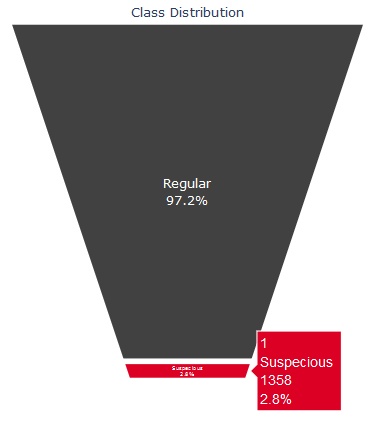
\includegraphics[width=.8\linewidth]{figures/class_imbalance.png}
    \caption{Class Distribution}
    \label{fig:class distribution}
\end{figure}

The complexity to build a model to detect a huge obstacle. In the features \ref{fig:Dimension reduction}
\begin{figure}[H]
    \centering
    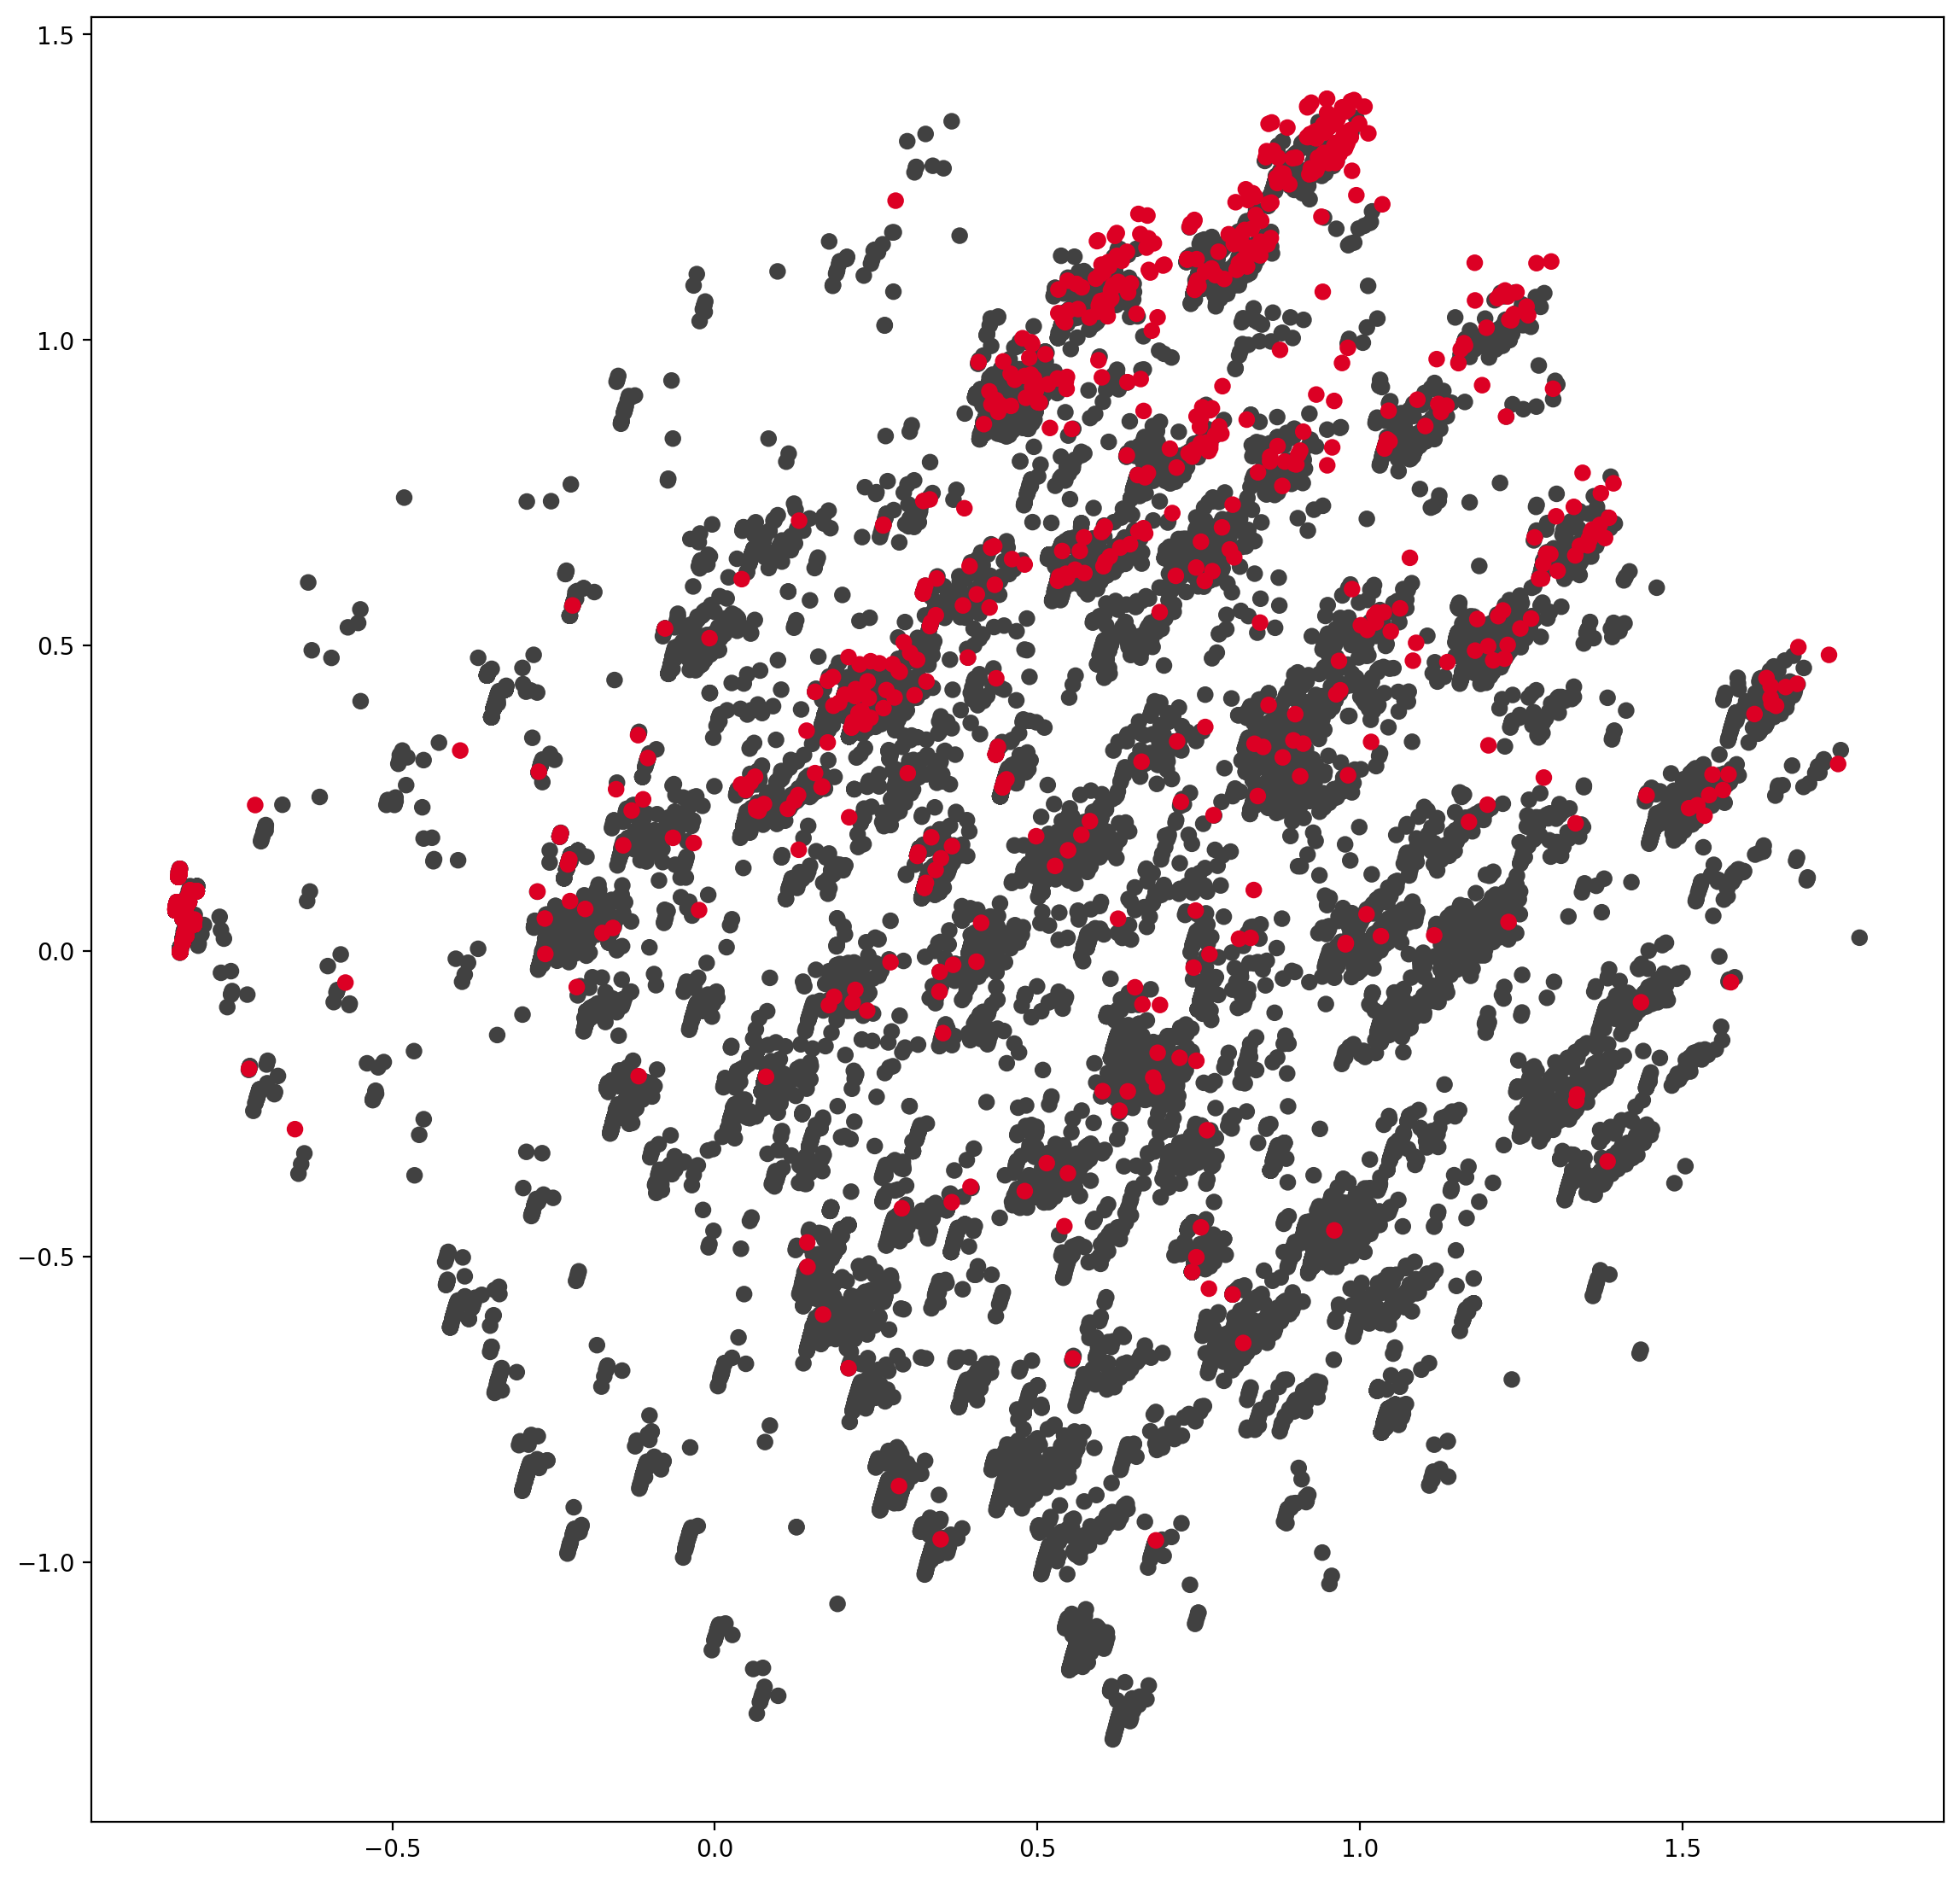
\includegraphics[width=\linewidth]{figures/pca_2d.png}
    \caption{Dimension reduction}
    \label{fig:Dimension reduction}
\end{figure}
The proportion of the fraudulent cases is shown in figure \ref{fig:feature proportion}. 
\begin{figure}[H]
    \centering
    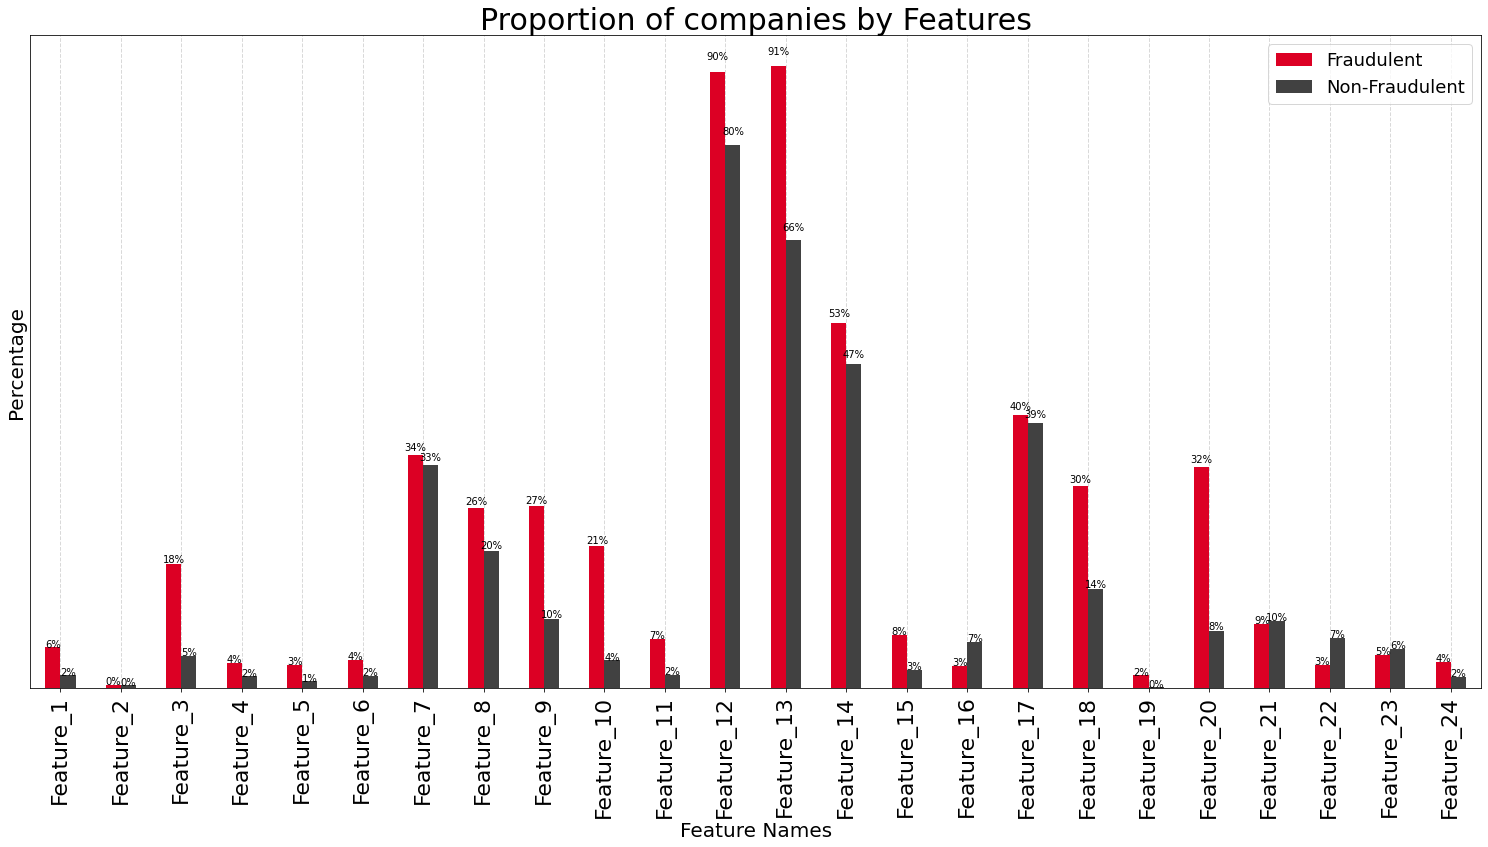
\includegraphics[width=\linewidth]{figures/feature_proportion.png}
    \caption{Proportion of binary features}
    \label{fig:feature proportion}
\end{figure}

\begin{figure}[H]
    \centering
    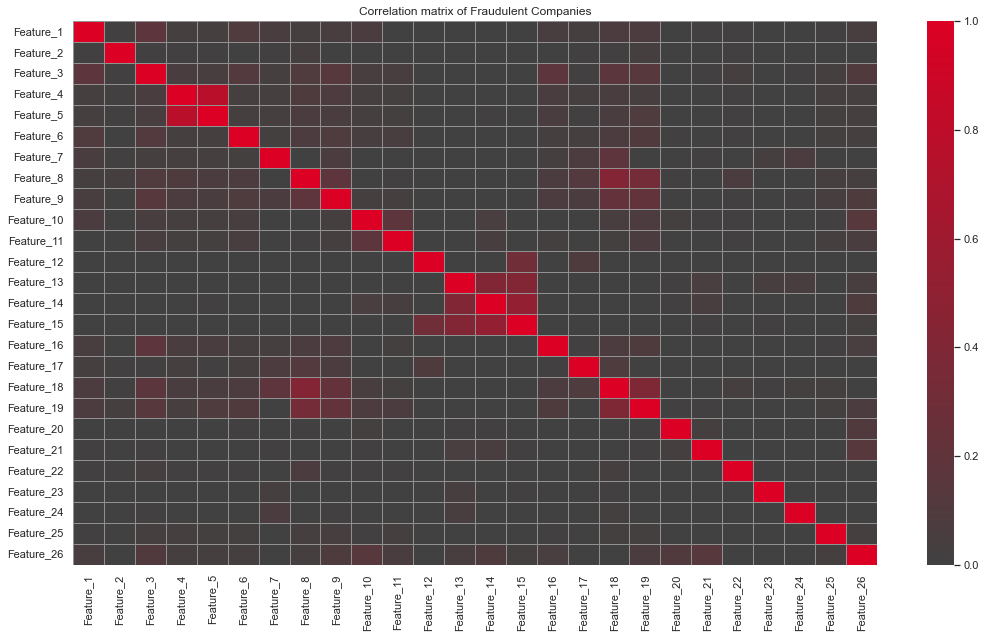
\includegraphics[width=\linewidth]{figures/corr.png}
    \caption{Correlation Matrix}
    \label{fig:corr}
\end{figure}

\subsubsection{Dataset Finalisation}\hspace*{\fill} \\
Finally the dataset has been segmented into train and test sets. From the
\begin{itemize}
    \item \textbf{Train and test split:}
    \item \textbf{Data Pre-processing:}
    \item \textbf{Handle class Imbalance:}
\end{itemize}

According to results shown in [] AUC values are stable or increased using class imbalanced and data driven method. 

\mytodo{show figure for AUC curve}


\begin{table}[h]
\begin{tabular}{@{}|l|l|l|l|l|l|@{}}
\toprule
\textbf{PCA} & \textbf{SMOTE} & \textbf{Model} & \textbf{Accuracy} & \textbf{Precision} & \textbf{Recall} \\ \midrule
\multirow{6}{*}{No}  & \multirow{3}{*}{No}  & \textbf{RF} & 0.0000 & 0.0000 & 0.0000 \\ \cmidrule(l){3-6} 
                     &                      & \textbf{XD} & 0.0000 & 0.0000 & 0.0000 \\ \cmidrule(l){3-6} 
                     &                      & \textbf{NN} & 0.0000 & 0.0000 & 0.0000 \\ \cmidrule(l){2-6} 
                     & \multirow{3}{*}{Yes} & \textbf{RF} & 0.0000 & 0.0000 & 0.0000 \\ \cmidrule(l){3-6} 
                     &                      & \textbf{XD} & 0.0000 & 0.0000 & 0.0000 \\ \cmidrule(l){3-6} 
                     &                      & \textbf{NN} & 0.0000 & 0.0000 & 0.0000 \\ \midrule
\multirow{6}{*}{Yes} & \multirow{3}{*}{No}  & \textbf{RF} & 0.0000 & 0.0000 & 0.0000 \\ \cmidrule(l){3-6} 
                     &                      & \textbf{XD} & 0.0000 & 0.0000 & 0.0000 \\ \cmidrule(l){3-6} 
                     &                      & \textbf{NN} & 0.0000 & 0.0000 & 0.0000 \\ \cmidrule(l){2-6} 
                     & \multirow{3}{*}{Yes} & \textbf{RF} & 0.0000 & 0.0000 & 0.0000 \\ \cmidrule(l){3-6} 
                     &                      & \textbf{XD} & 0.0000 & 0.0000 & 0.0000 \\ \cmidrule(l){3-6} 
                     &                      & \textbf{NN} & 0.0000 & 0.0000 & 0.0000 \\ \bottomrule
\end{tabular}
\caption{Model performance over test set}
\label{tab:model performance}
\end{table}

\begin{table}
    \begin{tabular}{lrrr}
\toprule
{} &  a &  b &  c \\
\midrule
0 &  1 &  3 &  4 \\
1 &  4 &  5 &  6 \\
\bottomrule
\end{tabular}

    \caption{Demo results}
    \label{tab:results}
\end{table}


\subsection{Method of Selection}
\mytodo{model selection hint\: https://medium.com/@matteding/imbalanced-data-fraud-detection-3185c1cdaa77}
\subsubsection{Confusion Matrix}\hspace*{\fill} \\
\mytodo{write how candonfusion matrix is used for model selection}
\subsubsection{AUC ROC}\hspace*{\fill} \\
\mytodo{how AUC ROC metrics are used}
\subsubsection{Threshold value}\hspace*{\fill} \\
\mytodo{Use of Threshold value to improve the model}